\chapter{Mengsels scheiden}\label{ch:g3:separating-mixtures}

Na een onweersbui zijn de plassen op straat bruin: regenwater gemengd met
aarde, zand en stukjes blad. Toch komt er helder water uit de kraan in
de keuken, en ook dat was ooit regen, voordat het in een rivier
terechtkwam. Hoe maak je modderwater weer schoon? Wat gemengd is, kun je
weer uit elkaar halen. Dit hoofdstuk laat zien hoe, de ene methode na de
andere.

\begin{recall}
\omterm{def:g2:mixing-and-dissolving:mix}{Mengen} is verschillende dingen bij elkaar doen. Een vaste stof zoals
suiker of zout \omterm{def:g2:mixing-and-dissolving:dissolve}{lost op} in water: hij verdwijnt uit het zicht, en de
heldere vloeistof is een oplossing. Een opgeloste vaste stof is er nog:
als het water opdroogt, blijft de vaste stof achter. Zand en aarde lossen
niet op (\cref{ch:g2:mixing-and-dissolving}).
\end{recall}

\section{Met de hand sorteren en zeven}

Als de stukjes van een mengsel groot genoeg zijn om te zien en op te
pakken, is de eenvoudigste manier om ze te scheiden met de hand: je kunt
de rozijnen een voor een uit de muesli halen. Zijn er te veel stukjes,
dan doet een zeef het sorteerwerk voor ons.

\begin{definition}[Zeven]\label{def:g3:separating-mixtures:sieve}
Bij \emph{zeven}\index{zeven} scheid je de stukjes van een mengsel op
grootte, met een zeef: een gaas of een plaat vol gaatjes. De kleine
stukjes vallen door de gaatjes; de grote stukjes blijven in de zeef
liggen.
\end{definition}

\begin{example}[Grind en zand]\label{ex:g3:separating-mixtures:gravel}
Een bouwvakker schudt een mengsel van grind en zand boven een zeef. Het
fijne zand valt erdoorheen op een hoop eronder; het grind blijft op het
gaas liggen.
\end{example}

\begin{omfigure}
\begin{tikzpicture}[font=\small]
  % the sieve: a mesh bowl
  \fill[pattern=crosshatch, pattern color=black!45] (-1.6,2.6) arc[start angle=180,
    end angle=360, x radius=1.6, y radius=0.7] -- cycle;
  \draw[black!70, line width=0.8pt] (-1.6,2.6) arc[start angle=180, end angle=360,
    x radius=1.6, y radius=0.7];
  \draw[black!70, line width=0.8pt] (-1.75,2.6) -- (1.75,2.6);
  \draw[black!70, line width=1.4pt] (1.75,2.6) -- (3.0,2.85);
  % gravel kept in the sieve
  \foreach \x/\y/\r in {-0.9/2.25/0.17,-0.45/2.12/0.2,0.05/2.08/0.18,0.5/2.13/0.21,
                        0.95/2.28/0.16,-0.2/2.42/0.15,0.3/2.43/0.17}
    \fill[black!45, draw=black!65] (\x,\y) circle (\r);
  % sand falling
  \foreach \x/\y in {-0.4/1.6,0.1/1.4,0.4/1.7,-0.15/1.15,0.25/1.0,-0.5/0.95,0.0/0.75}
    \fill[orange!60!brown] (\x,\y) circle (0.05);
  % the heap of sand in a bowl
  \fill[orange!45!brown!70] (-1.0,0.12) .. controls (-0.5,0.55) and (0.5,0.55)
    .. (1.0,0.12) -- cycle;
  \draw[black!70, line width=0.8pt] (-1.5,0.5) .. controls (-1.3,0) and (1.3,0)
    .. (1.5,0.5);
  \node[anchor=west] at (2.0,2.2) {het grind blijft in de zeef};
  \node[anchor=west] at (2.0,1.25) {het zand valt door de gaatjes};
  \node[anchor=west] at (2.0,0.3) {een hoopje zand};
\end{tikzpicture}

{\small Een mengsel van grind en zand \omterm{def:g3:separating-mixtures:sieve}{zeven}: de stukjes worden op grootte
gesorteerd.}
\end{omfigure}

\begin{omfigure}
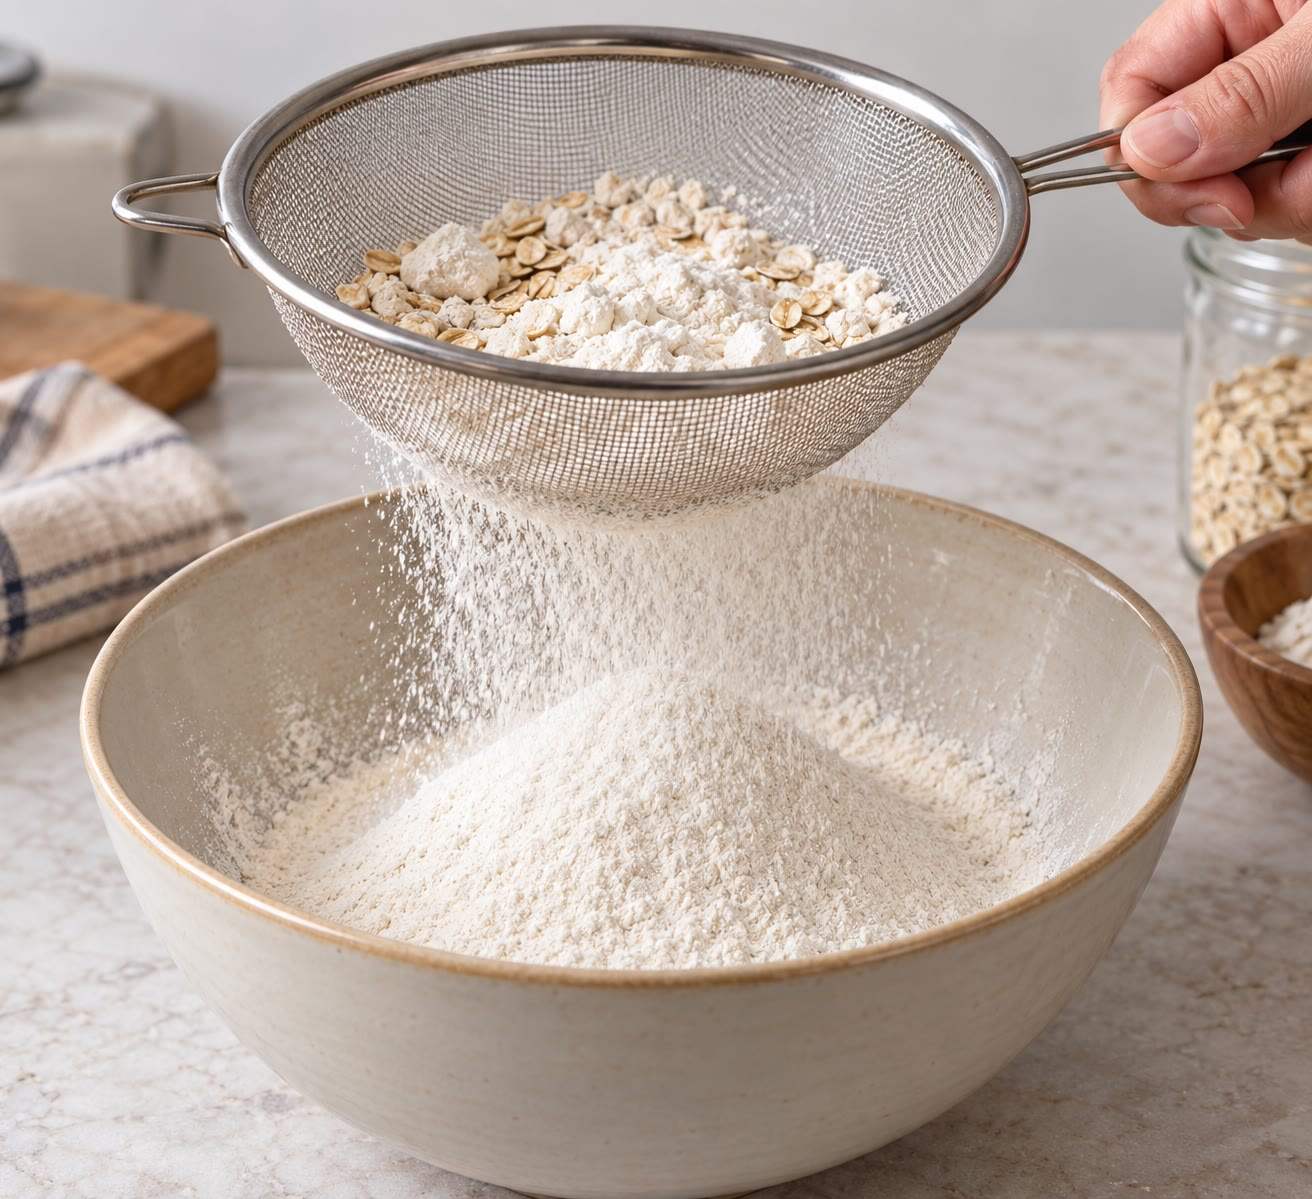
\includegraphics[width=0.55\linewidth]{images/book1/ai/g3-kitchen-sieve.jpg}

{\small Een keukenzeef: het fijne meel gaat erdoor, de klontjes blijven
achter.}
\end{omfigure}

\section{Laten bezinken en afschenken}

\begin{definition}[Bezinken en afschenken]\label{def:g3:separating-mixtures:decant}
Een mengsel van water en een vaste stof die niet \omterm{def:g2:mixing-and-dissolving:dissolve}{oplost}, kun je laten
staan: de vaste stof zakt langzaam naar de bodem. Dat heet
\emph{bezinken}\index{bezinken}. Als alles bezonken is, kun je het
heldere water erboven voorzichtig in een ander bakje gieten, terwijl de
vaste stof achterblijft: dat is \emph{afschenken}\index{afschenken}.
\end{definition}

\begin{omfigure}
\begin{tikzpicture}[font=\small]
  % 1: stirred, cloudy
  \pic at (0,0) {beaker={0.7}{brown!28}};
  \foreach \x/\y in {-0.5/0.3,-0.2/0.6,0.3/0.4,0.5/0.9,-0.4/1.0,0.1/1.2,0.4/0.15,
                     -0.1/0.25,0.2/0.8,-0.55/0.7}
    \fill[brown!60] (\x,\y) circle (0.03);
  \node[anchor=north, align=center] at (0,-0.15) {geroerd:\\ troebel};
  \draw[->, thick, omProp] (1.1,1.0) -- (2.4,1.0);
  % 2: settled
  \pic at (3.5,0) {beaker={0.7}{omWater!80}};
  \fill[brown!60] (2.7,0) rectangle (4.3,0.25);
  \draw[omGlass, line width=0.7pt] (2.7,0.25) -- (2.7,0) -- (4.3,0) -- (4.3,0.25);
  \node[anchor=north, align=center] at (3.5,-0.15) {laten staan:\\ de aarde is bezonken};
  \draw[->, thick, omProp] (4.6,1.0) -- (5.9,1.0);
  % 3: decanted
  \pic at (7.0,0) {beaker={0.1}{omWater!80}};
  \fill[brown!60] (6.2,0) rectangle (7.8,0.25);
  \draw[omGlass, line width=0.7pt] (6.2,0.25) -- (6.2,0) -- (7.8,0) -- (7.8,0.25);
  \pic at (9.2,0) {beaker={0.58}{omWater!80}};
  \node[anchor=north, align=center] at (8.1,-0.15) {afgeschonken: helder water\\ rechts, de aarde blijft achter};
\end{tikzpicture}

{\small Een mengsel van aarde en water laten \omterm{def:g3:separating-mixtures:decant}{bezinken} en daarna
\omterm{def:g3:separating-mixtures:decant}{afschenken}.}
\end{omfigure}

\begin{remark}[Bezinken kost tijd]\label{rem:g3:separating-mixtures:time}
Grote, zware korrels \omterm{def:g3:separating-mixtures:decant}{bezinken} in een paar minuten; heel fijne klei kan
er een dag of langer over doen, en zolang blijft het water een beetje
troebel. \omterm{def:g3:separating-mixtures:decant}{Afschenken} haalt nooit elk korreltje weg: een beetje troebeling
gaat met het water mee.
\end{remark}

\section{Filtreren}

\begin{definition}[Filtreren en filtraat]\label{def:g3:separating-mixtures:filter}
Bij \emph{filtreren}\index{filtreren} giet je een mengsel door een
filter: een vel papier, een doek of een laag zand met gaatjes die te
klein zijn om de vaste stukjes door te laten. De vaste stof blijft op
het filter liggen; de heldere vloeistof die erdoorheen gaat, heet het
\emph{filtraat}\index{filtraat}.
\end{definition}

\begin{omfigure}
\begin{tikzpicture}[font=\small, scale=1.4]
  \pic[transform shape] at (0,0) {beaker={0.35}{omWater!80}};
  \pic[transform shape] at (0,1.4) {funnel={brown!55}};
  % muddy water waiting in the paper cone, above the soil
  \fill[brown!25] (-0.411,2.45) -- (0.411,2.45) -- (0.722,2.8) -- (-0.722,2.8) -- cycle;
  % drops of filtrate
  \foreach \y in {1.15,0.95} \fill[omDef!50] (0,\y) circle (0.04);
  \draw[<-, omProp, thick] (0.75,2.6) -- (2.0,2.9) node[right, text=black]
    {filtreerpapier in een trechter};
  \draw[<-, omProp, thick] (0.25,2.15) -- (2.0,2.2) node[right, text=black]
    {de aarde blijft op het papier};
  \draw[<-, omProp, thick] (0.85,0.4) -- (2.0,0.6) node[right, text=black]
    {het filtraat: helder water};
\end{tikzpicture}

{\small Modderwater \omterm{def:g3:separating-mixtures:filter}{filtreren} door een papieren filter.}
\end{omfigure}

\begin{inthelab}[Modderwater filtreren]
De docent vouwt een rond vel filtreerpapier tot een kegel en zet die in
een glazen trechter boven een bekerglas. Het modderwater wordt beetje bij
beetje in de kegel gegoten, nooit boven de rand van het papier. Er
druppelt helder water in het bekerglas; de aarde vormt een bruine laag
op het papier. Is het \omterm{def:g3:separating-mixtures:filter}{filtraat} troebel, dan is het papier gescheurd of
is het water over de rand gelopen.
\end{inthelab}

\begin{proposition}[Een filter houdt niet tegen wat opgelost is]\label{prop:g3:separating-mixtures:dissolved}
Een filter houdt de vaste stukjes tegen die niet opgelost zijn. Wat
opgelost is, houdt het niet tegen: zout water dat je door een filter
giet, komt er net zo zout uit, en zoete thee net zo zoet.
\end{proposition}

\begin{omfigure}
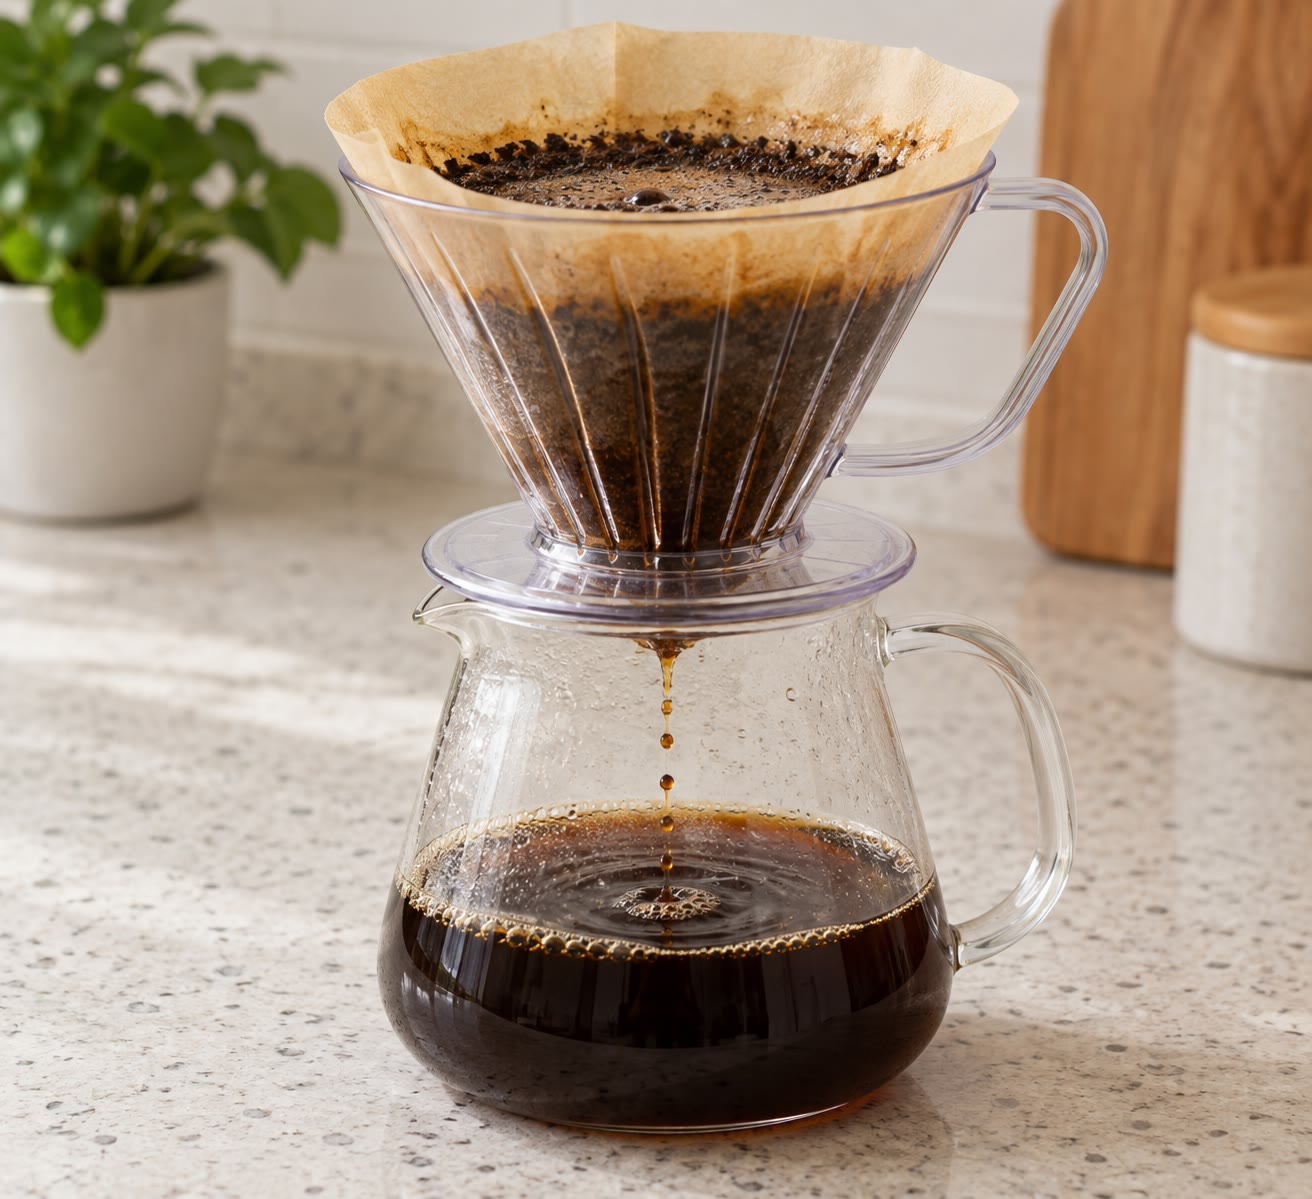
\includegraphics[width=0.5\linewidth]{images/book1/ai/g3-coffee-filter.jpg}

{\small Koffie zetten is \omterm{def:g3:separating-mixtures:filter}{filtreren}: het koffiedik blijft in het papier,
de koffie is het \omterm{def:g3:separating-mixtures:filter}{filtraat}.}
\end{omfigure}

\section{Het water laten verdampen}

\begin{definition}[Indampen]\label{def:g3:separating-mixtures:evaporate}
Om een vaste stof die in water opgelost is terug te krijgen, laat je het
water opdrogen, in de zon of op een zacht vuurtje: dat is
\emph{indampen}\index{indampen}. Het water gaat de lucht in; de vaste
stof blijft in het schaaltje.
\end{definition}

\begin{example}[Zout uit zout water]\label{ex:g3:separating-mixtures:salt}
Een beetje zout water wordt in een ondiep schaaltje gegoten en op een
zonnige vensterbank gezet. Dagen later is er geen water meer over, alleen
een wit korstje zout: het zout dat opgelost was.
\end{example}

\begin{omfigure}
\begin{tikzpicture}[font=\small, scale=1.4]
  \pic[transform shape] at (0,0) {hotplate};
  \pic[transform shape] at (0,0) {evapdish={omWater!80}};
  \node[anchor=north, align=center] at (0,-0.6) {zout water,\\ zacht verwarmd};
  \draw[->, thick, omProp] (1.5,0.3) -- (3.0,0.3) node[midway, above, text=black]
    {later};
  \pic[transform shape] at (4.5,0) {hotplate};
  \pic[transform shape] at (4.5,0) {evapdish={white!85!black}};
  \foreach \x in {-0.45,-0.25,-0.05,0.15,0.35}
    \fill[white, draw=black!45, line width=0.2pt] (4.5+\x,0.12) rectangle ++(0.09,0.06);
  \node[anchor=north, align=center] at (4.5,-0.6) {geen water meer:\\ zoutkristallen};
  \foreach \x in {-0.3,0,0.3} \draw[->, black!45, decorate,
    decoration={snake, amplitude=0.6pt, segment length=4pt}] (\x,0.7) -- (\x,1.4);
  \node[anchor=south] at (0,1.4) {water gaat de lucht in};
\end{tikzpicture}

{\small \omterm{def:g3:separating-mixtures:evaporate}{Indampen} in het laboratorium: de docent verwarmt het schaaltje
zachtjes op een kookplaat. Het zout blijft in het schaaltje.}
\end{omfigure}

\section{Welke methode voor welk mengsel?}

\begin{method}[Een scheidingsmethode kiezen]\label{met:g3:separating-mixtures:choose}
Om een mengsel uit elkaar te halen, vraag je je af:
\begin{enumerate}
  \item Zijn de stukjes groot en verschillend van grootte? Sorteer met
        de hand, of zeef.
  \item Zit er een vaste stof die niet \omterm{def:g2:mixing-and-dissolving:dissolve}{oplost} in een vloeistof? Laat
        \omterm{def:g3:separating-mixtures:decant}{bezinken} en schenk af, of filtreer voor helderder water.
  \item Is er een vaste stof in de vloeistof opgelost? Damp de vloeistof
        in: de vaste stof blijft achter.
\end{enumerate}
Vaak zijn er meerdere stappen nodig, de ene na de andere.
\end{method}

\begin{example}[Zand, zout en water]\label{ex:g3:separating-mixtures:three}
In een pot zit water met zand en zout erin. Het zout is opgelost, het
zand niet.
\begin{enumerate}
  \item Filtreer: het zand blijft op het papier.
  \item Het \omterm{def:g3:separating-mixtures:filter}{filtraat} is helder, maar het is zout water. Damp het in: het
        zout blijft in het schaaltje.
\end{enumerate}
Twee methoden, de ene na de andere, geven het zand en het zout terug.
\end{example}

\begin{example}[Schoon water uit een rivier]\label{ex:g3:separating-mixtures:plant}
Een waterzuiveringsinstallatie maakt rivierwater in een paar stappen
drinkbaar:
\begin{enumerate}
  \item het rivierwater gaat door roosters, grote hekken die takken,
        bladeren en plastic tegenhouden: een soort zeven;
  \item het staat stil in grote bassins, waar het slib naar de bodem
        zakt;
  \item het wordt gefiltreerd door dikke lagen zand die de fijnste
        korreltjes tegenhouden;
  \item er komt een heel klein beetje van een middel bij dat ziektekiemen
        doodt, zodat het water in de leidingen veilig blijft.
\end{enumerate}
\end{example}

\begin{omfigure}
\begin{tikzpicture}[font=\small, node distance=0.45cm,
    box/.style={draw=omDef, fill=omDef!6, rounded corners=2pt, align=center,
      minimum height=1.15cm, text width=2.0cm}]
  \node[box] (r) {rivier-\\ water};
  \node[box, right=of r] (s) {roosters\\ (zeven)};
  \node[box, right=of s] (t) {bezink-\\ bassins};
  \node[box, right=of t] (f) {zand-\\ filters};
  \node[box, right=of f] (g) {kiemen\\ gedood};
  \foreach \a/\b in {r/s,s/t,t/f,f/g} \draw[->, thick, omProp] (\a) -- (\b);
  \node[below=0.15cm of s, font=\footnotesize, align=center] {takken,\\ plastic};
  \node[below=0.15cm of t, font=\footnotesize, align=center] {slib};
  \node[below=0.15cm of f, font=\footnotesize, align=center] {fijne korreltjes};
  \draw[->, thick, omProp] (g.south) -- ++(0,-0.8) node[below] {naar de kranen};
\end{tikzpicture}

{\small De stappen van een waterzuiveringsinstallatie. Onder elke stap:
wat die stap weghaalt.}
\end{omfigure}

\begin{omfigure}
\begin{minipage}[t]{0.48\linewidth}\centering
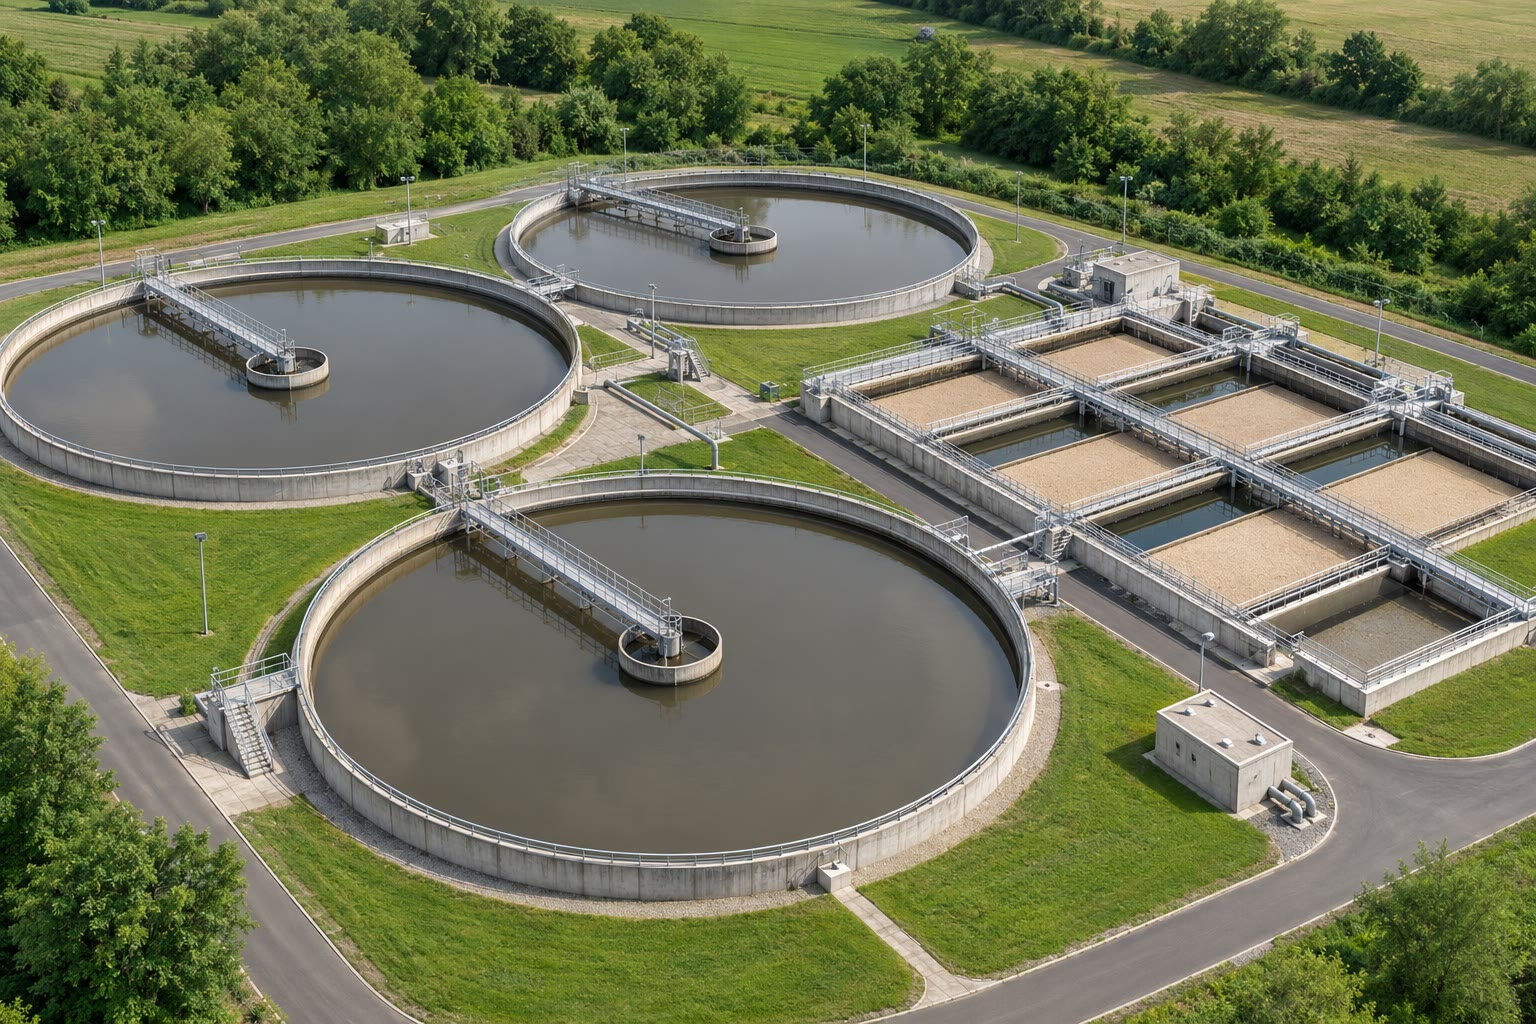
\includegraphics[width=\linewidth,height=4.6cm,keepaspectratio]{images/book1/ai/g3-settling-tanks.jpg}

{\small Bezinkbassins van een waterzuiveringsinstallatie.}
\end{minipage}\hfill
\begin{minipage}[t]{0.48\linewidth}\centering
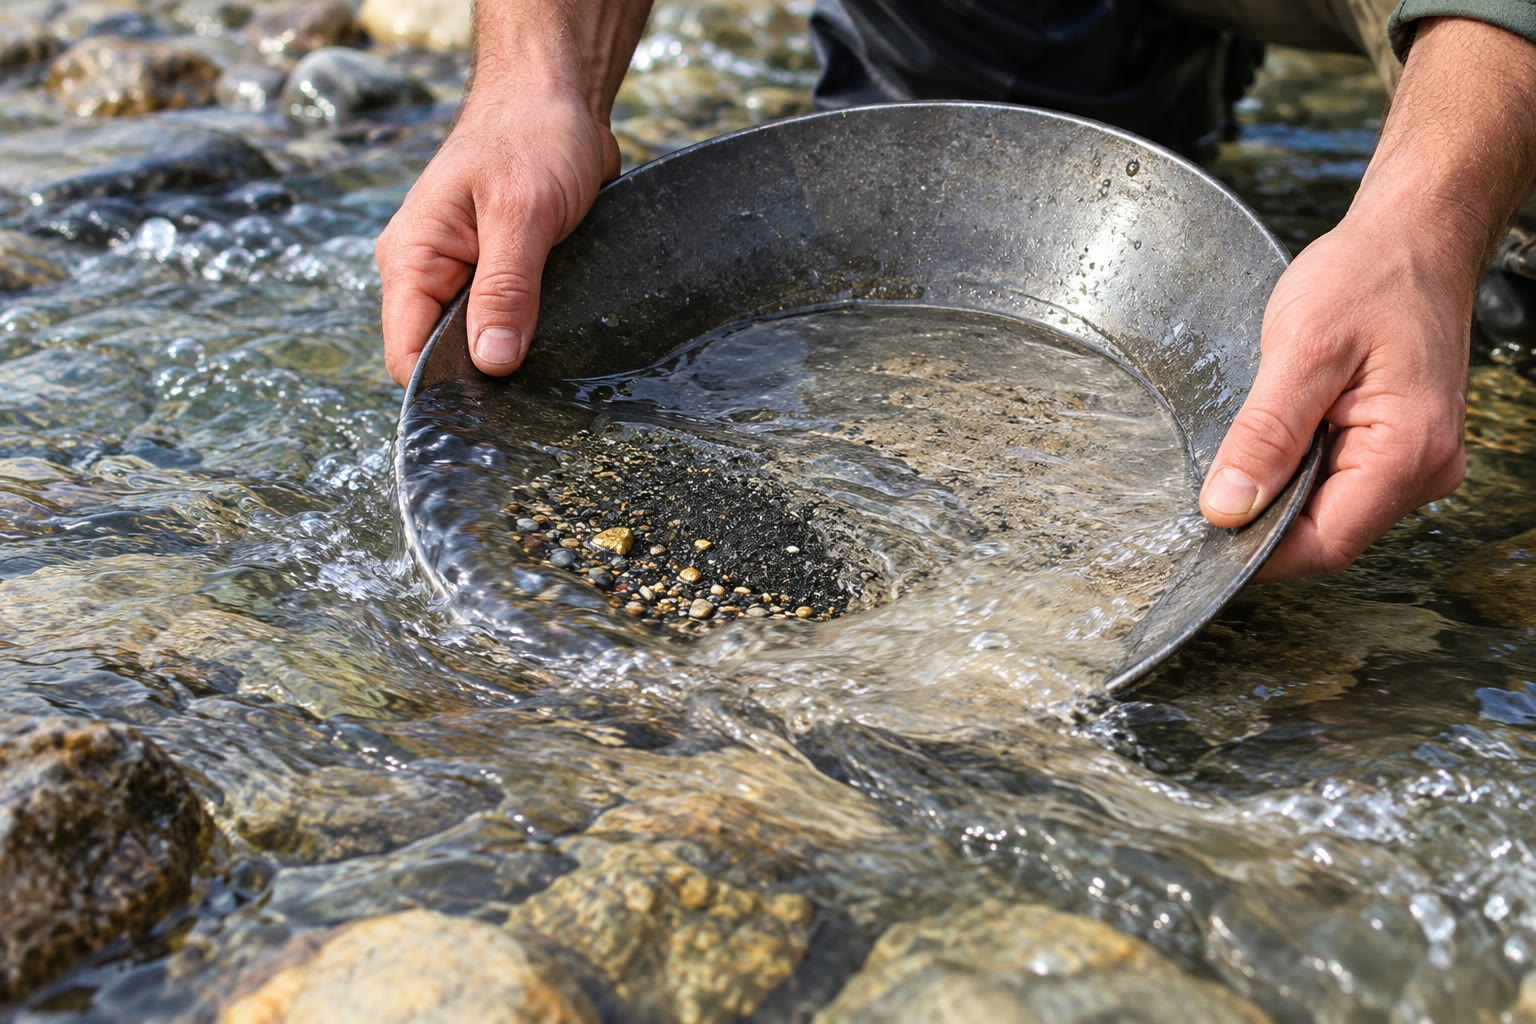
\includegraphics[width=\linewidth,height=4.6cm,keepaspectratio]{images/book1/ai/g3-gold-panning.jpg}

{\small Goudzoeken met een pan: het rivierwater voert het lichte zand
mee; de zware korrels blijven in de pan.}
\end{minipage}
\end{omfigure}

\begin{remark}[Helder is niet altijd schoon]\label{rem:g3:separating-mixtures:clean}
Gefiltreerd water kan er volkomen helder uitzien en toch opgeloste
stoffen bevatten, en ziektekiemen die veel te klein zijn om te zien.
Daarom drinkt niemand water uit een plas of een beek, ook niet nadat het
gefiltreerd is.
\end{remark}

\section{Oefeningen}

\begin{exercise}[$\star$]\label{exo:g3:separating-mixtures:1}
Welke methode zou je gebruiken om erwten van rijstkorrels te scheiden?
\end{exercise}

\begin{exercise}[$\star$]\label{exo:g3:separating-mixtures:2}
Een glas modderwater blijft een uur op tafel staan. Wat gebeurt er met
de aarde? Hoe heet dat?
\end{exercise}

\begin{exercise}[$\star$]\label{exo:g3:separating-mixtures:3}
Wat is een \omterm{def:g3:separating-mixtures:filter}{filtraat}? Wat is het \omterm{def:g3:separating-mixtures:filter}{filtraat} als je koffie zet?
\end{exercise}

\begin{exercise}[$\star$]\label{exo:g3:separating-mixtures:4}
Zout water wordt door filtreerpapier gegoten. Is het \omterm{def:g3:separating-mixtures:filter}{filtraat} zout?
Leg uit.
\end{exercise}

\begin{exercise}[$\star$]\label{exo:g3:separating-mixtures:5}
Hoe kun je de suiker terugkrijgen uit een glas suikerwater?
\end{exercise}

\begin{exercise}[$\star$]\label{exo:g3:separating-mixtures:6}
Kijk naar de figuur van de zeef. Welke stukjes blijven in de zeef? Waarom
vallen de andere erdoorheen?
\end{exercise}

\begin{exercise}[$\star$]\label{exo:g3:separating-mixtures:7}
Zoek bij elk mengsel een methode --- \omterm{def:g3:separating-mixtures:sieve}{zeven}, \omterm{def:g3:separating-mixtures:filter}{filtreren} of \omterm{def:g3:separating-mixtures:evaporate}{indampen}:
(a) zand en kiezels; (b) krijtpoeder in water; (c) zout in water.
\end{exercise}

\begin{exercise}[$\star$]\label{exo:g3:separating-mixtures:8}
Kijk naar de figuur van de waterzuiveringsinstallatie. Door hoeveel
stappen gaat het water? Welke stap haalt het slib weg?
\end{exercise}

\begin{exercise}[$\star$]\label{exo:g3:separating-mixtures:9}
Zet deze stappen in de goede volgorde om het zand en het zout terug te
krijgen uit een pot met zand, zout en water: het \omterm{def:g3:separating-mixtures:filter}{filtraat} \omterm{def:g3:separating-mixtures:evaporate}{indampen};
\omterm{def:g3:separating-mixtures:filter}{filtreren}; het zand van het papier halen.
\end{exercise}

\begin{exercise}[$\star\star$]\label{exo:g3:separating-mixtures:10}
Kan een filter zeewater drinkbaar maken? Leg uit waarom niet.
\end{exercise}

\begin{exercise}[$\star\star$]\label{exo:g3:separating-mixtures:11}
In een theepot vol thee liggen nog theeblaadjes. Noem twee methoden uit
dit hoofdstuk die de thee van de blaadjes scheiden.
\end{exercise}
